\subsection{Distribuição cadastral e evidência de integração}\label{sec:mapa-artesp}
A Figura~\ref{fig:mapa-artesp} representa as 337 coordenadas existentes no recorte auditado, sem geocodificação ou deslocamento editorial dos pontos. A malha é a municipal IBGE 2024, código 3529401, utilizada na contagem; não foi substituída por um limite simplificado. As estações são símbolos separados e não integram o total das paradas ARTESP. A distribuição é desigual no território e não permite calcular população coberta, acessibilidade física ou disponibilidade operacional.
\begin{figure}[H]\centering
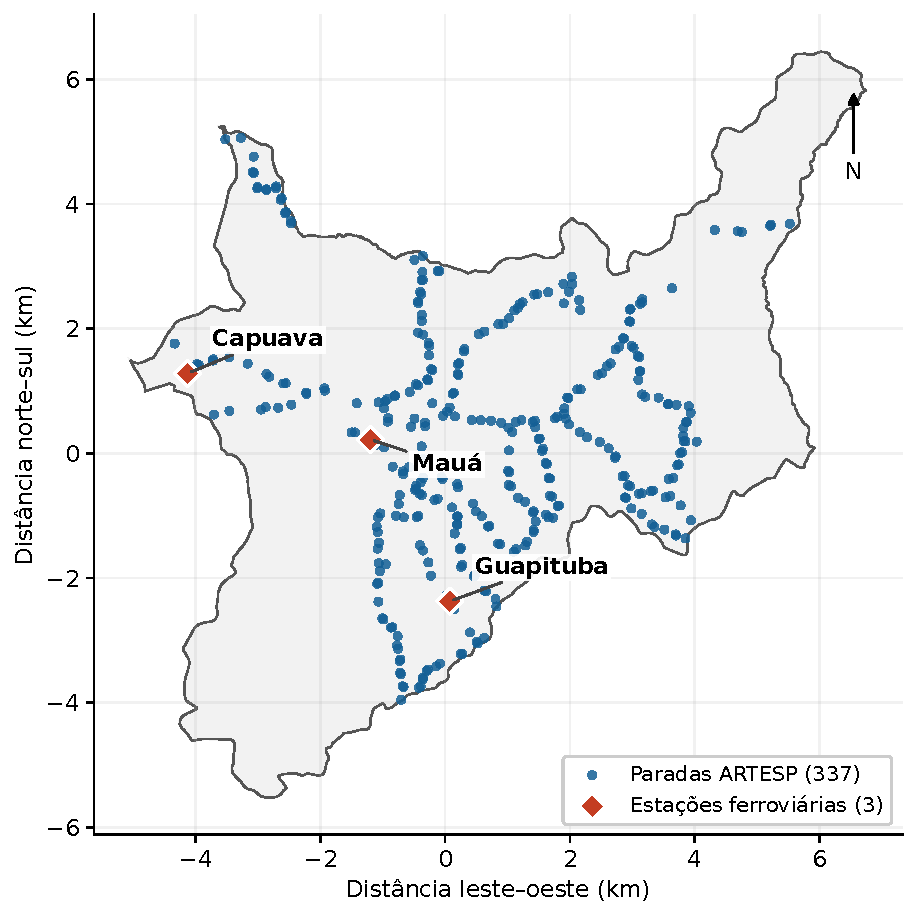
\includegraphics[width=.95\textwidth]{revisao-tecnico-cientifica-2026-11-02/mapa-artesp-maua.pdf}
\caption{Distribuição das paradas ARTESP auditadas e das estações ferroviárias em Mauá.}\label{fig:mapa-artesp}
\fonte{Coordenadas de \nolinkurl{stops.csv} e \nolinkurl{summary.json}; malha \nolinkurl{maua-ibge-2024.geojson}, SIRGAS 2000, auditoria de 2 nov. 2026. Eixos em aproximação métrica local, origem em $(-23{,}67; -46{,}45)$; não representam distância de caminhada.}
\end{figure}
\begin{figure}[H]\centering
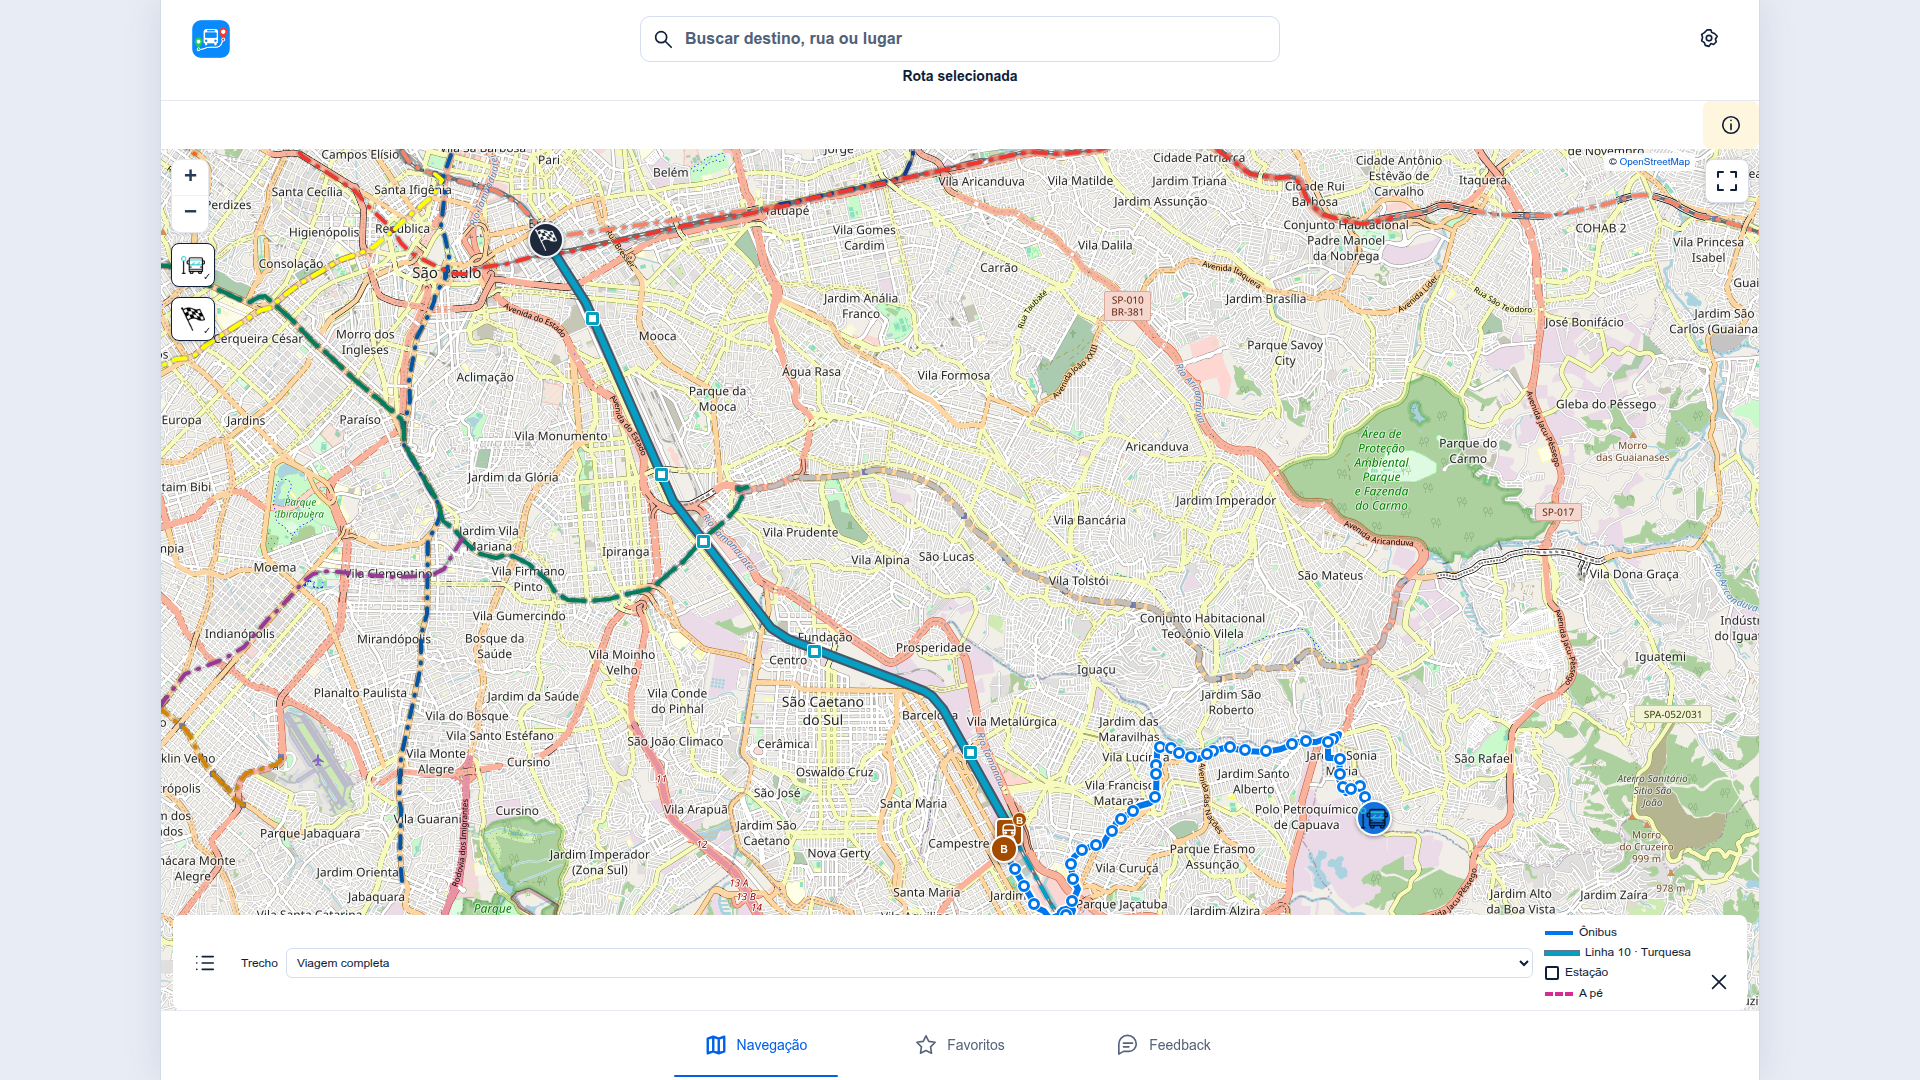
\includegraphics[width=\textwidth,trim=160bp 0 160bp 0,clip]{auditoria-artesp-maua-2026-11-02/captura-maua-bras-mapa.png}
\caption{Consulta Oscarito--Brás com ônibus ARTESP 157 e CPTM Linha 10--Turquesa.}\label{fig:artesp-onibus-trem}
\fonte{Captura da interface em 2 nov. 2026, por volta de 02h19; acervo \nolinkurl{auditoria-artesp-maua-2026-11-02/}. Consulta parcial, com chegada planejada às 06h26; não é uma viagem observada.}
\end{figure}
A Figura~\ref{fig:artesp-onibus-trem} já existia no acervo e demonstra a composição das modalidades na interface. O aviso de busca parcial, visível no painel da Figura~\ref{fig:artesp-consulta-detalhe}, faz parte da evidência e foi mantido. Esta consulta de madrugada não corresponde às consultas das 08h da Tabela~\ref{tab:artesp-maua-consultas}; sua presença não permite substituir resultados, comparar durações entre horários distintos ou afirmar ótimo global. Foram retiradas apenas as margens laterais vazias na diagramação; a imagem original foi preservada. O detalhe da alternativa está na Figura~\ref{fig:artesp-consulta-detalhe}.

\begin{figure}[H]\centering
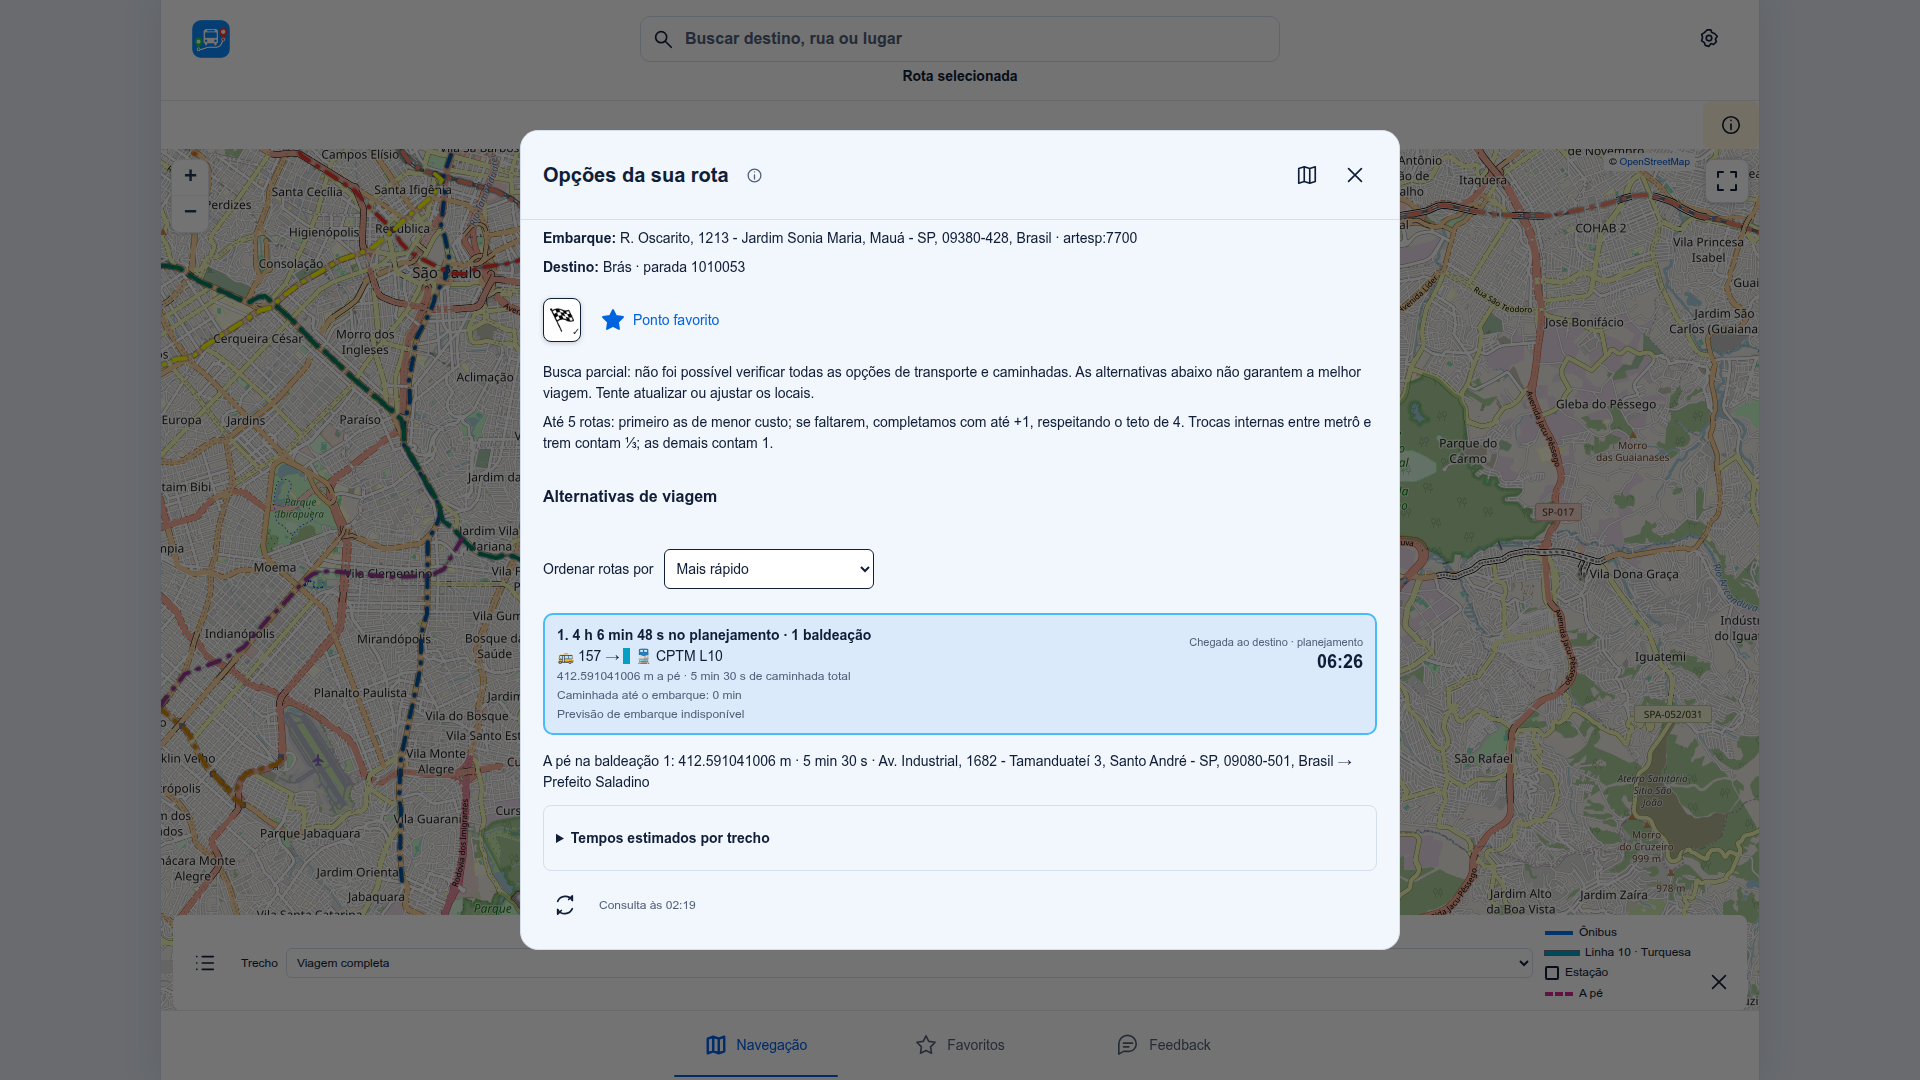
\includegraphics[width=\textwidth,trim=520bp 130bp 520bp 130bp,clip]{auditoria-artesp-maua-2026-11-02/captura-maua-bras-consulta.png}
\caption{Alternativa ônibus--ferrovia e aviso de busca parcial na consulta de madrugada.}\label{fig:artesp-consulta-detalhe}
\fonte{Recorte ampliado do painel da mesma sessão da Figura~\ref{fig:artesp-onibus-trem}, em 2 nov. 2026. Programação e estimativas; não há previsão operacional ARTESP.}
\end{figure}
